\chapter{II. IDENTIFICACIÓN DEL PROBLEMA }
\section{Descripción de la situación problemática}
“El sector turístico es uno de los sectores económicos que han experimentado una evolución mayor en los últimos tiempos. Cabe destacar la transformación sustancial que se ha producido en las preferencias y el comportamiento de los turistas, dejando a un lado los paquetes turísticos pre-organizados que ofrecen los intermediarios turísticos a favor de otras opciones más personalizadas, provocando que la planificación de un viaje se convierta en una tarea compleja.(Uriel \& Hernández, 2004; Hyde \& Lawson, 2003)” \cite{RodriguezDiaz2012SistemaPersonalizado}. 

Un turista que desea visitar un destino de sin depender de opciones pre-diseñadas lleva consigo la tarea de planificar por su propia cuenta un itinerario de viaje, para ello primeramente una vez que tiene el destino busca información. En la actualidad se puede acceder a bastante información en la internet, en las que se pueden encontrar guías, en blogs, páginas de entidades del estado que brindan información de los destinos, los comentarios de otros respecto a lugar, actividad y hospedajes que desea visitar en las que encontramos a Tripadvisor, poder elegir y reservar hospedajes en aplicaciones populares de Tripadvisor, Booking, Trivago y Airbnb, También herramientas como Google Maps en la cual se pueden visualizar formas de acceder al lugar, servicios cerca de un lugar específico, entre otra información gracias al crecimiento de la internet. Está tarea de buscar información puede convertirse tediosa por la gran cantidad de información disponible.

En segundo lugar decidir tiene que decidir de acuerdo a sus preferencias y las restricciones del lugar para realizar un plan que incluye un itinerario en las que dependiendo incluye por día las actividades que realizará, precios, información del lugar, reservas de hospedajes y transporte, con los tiempos requeridos por cada punto de interés(PDI). Esta tarea puede convertirse en una tarea compleja que demande un alto costo en tiempo y esfuerzo para evaluar todas las alternativas, que al final no le garantiza tener el mejor itinerario.

Además si buscamos tener una buena solución aumentamos la complejidad ya que encontramos teorías como al tener en cuenta las decisiones en la planificación según \cite{Ehrgott2005MulticriteriaOptimization} las decisiones generalmente involucran objetivos conflictivos, y para resolver de manera óptima tienen que ser resueltas según criterios. Considerando esto \cite{RodriguezDiaz2012SistemaPersonalizado} identificó que los objetivos en conflictos que tiene el turista al diseñar su propio viaje son minimizar costes, maximizar las satisfacción al realizar actividades. 

Al buscar soluciones que devuelvan una solución confiable, encontramos que es posible modelar matemáticamente en la cual podemos tener una solución mejor, apoyándose del poder de las computadores. Al intentar solucionar de forma exacta y rápida no es posible solucionar por la gran cantidad de variables(numero de actividades a realizar en el destino) que se tiene en el momento de la planificación, Según \citeA{RodriguezDiaz2012SistemaPersonalizado} es presentado como un problema de rutas, de asignación de actividades y multicriterio. El problema de construir un itinerario de viaje es también considerado como una variante del problema del Agente Viajero el cual es uno de los problemas de tipo NP-Hard como uno de los problemas que no se puede encontrar una solución con un coste computacional y tiempo razonable. 

Puno se encuentra en el cuarto lugar de los departamentos del Perú mas visitados por turistas extranjeros en el 2017 según un reporte publicado por \citeA{2017PerfilExtranjero}.  “Puno es sin lugar a dudas uno de los destinos más atractivos del Perú y uno de los más interesantes en el continente: pocas ciudades tienen el privilegio de ubicarse a orillas de una maravilla de la naturaleza como el Lago Titicaca, el lago navegable más alto del mundo a más de 3800 msnm.”  \cite{TurismoPuno}.

Se ha observado que a nivel nacional no existe una solución tal como lo indica \citeA{mendoza2017diseno} en su Tesis realizado en la Región Puno “Revisando los sitios web oficiales y más promocionados por el Ministerio de Comercio Exterior y Turismo (MINCETUR) como son: www.peru.travel, www.ytuqueplanes.com, www.turismoruralcomunitario.com.pe, se advierte que no cuentan con un componente que integre un modelo matemático para la toma de decisiones, que sea capaz de evaluar todas las diferentes alternativas con una determinada cantidad de variables, con el objetivo de diseñar un viaje a medida según las preferencias y necesidades del turista; afirmación que es también corroborada por el representante del Turismo Rural Comunitario en la Región Puno.” 

Se considera una gran oportunidad el implementar un modelo matemático para el problema de diseñar un itinerario de viaje detallado en la que se tenga como resultado una ruta detallada por día con actividades a realizar en la considere los criterios como es minimizar los costes y maximizar la satisfacción, las restricciones del lugar, las preferencias del turista en la región de Puno.

\section{Objetivos de la investigación}

\subsection{Objetivo general}
Desarrollar una herramienta que proporcione a cada turista un itinerario detallado de viaje de acuerdo a sus preferencias del turista y las restricciones del lugar, que incluye las actividades que puede realizar en un horario establecido.

\subsection{Objetivos específicos}
\begin{itemize}
\item Diseñar e implementar la heurística de construcción El vecino más cercano y la heurística de mejoría 2-opt y/o otros, utilizado el lenguaje de programación Python.
\item Implementar la Metaheurística Búsqueda Tabú para mejorar la solución de la heurística de mejoría, utilizado Python.
\item Validar el algoritmo con técnicas estadísticas utilizando instancias artificiales encontradas en la literatura y datos reales de la región Puno.
\item Desarrollar una aplicación web que permita al turista ingresar sus preferencias y visualizar el itinerario detallado utilizando el framework web Django y Api de Google Maps.
\end{itemize}
\section{Justificación}
“El turismo, en muchos países en desarrollo y menos adelantados, es la opción de desarrollo económico más viable y sostenible y, en algunos de ellos, la principal fuente de entrada de divisas. Parte de estos ingresos revierte en diferentes grupos de la sociedad y, si el turismo se gestiona centrándose prioritariamente en la atenuación de la pobreza, puede beneficiar directamente a los grupos más pobres mediante el empleo de la población local en empresas turísticas, el suministro de bienes y servicios a los turistas, la gestión de pequeñas empresas y empresas comunitarias, etc., con el consecuente impacto positivo en la reducción de la pobreza”. \cite{ElPobreza}.

“El Perú es un país en el que hasta el año 2013 el 20.7\% de sus habitantes se encontraba en condición de pobreza, siendo Cajamarca y Huancavelica las regiones que registran los mayores índices. Además de las regiones mencionadas, de acuerdo con el Instituto Nacional de Estadística (INEI), Amazonas, Apurímac, Ayacucho, Huánuco, Loreto, Pasco, Piura y Puno se encuentran en la lista de las que tienen la mayor cantidad de personas con más bajos recursos económicos. Las jurisdicciones donde se observan los mayores indicadores de pobreza son, paradójicamente, las que menos están invirtiendo en proyectos sociales.” \cite{2017RegionesPeru21}. 

De acuerdo al último reporte en la actualidad publicado por Promperú titulado “Perfil del Turista Extranjero que visita Puno (2016)” aproximadamente 612 000 turistas extranjeros visitaron la región de Puno en 2016 de la cuales 66\% de os turistas viajan por cuenta propia (sin utilizar los servicios de una agencia de viajes/turismo) como se puede observar en la Figura~\ref{fig:modalidad_viaje_extrajero}. Así mismo el 67\% de ellos utilizan internet como medio que más influye en la elección de un destino, y también se observa que el 81\% planifica su viaje.
\begin{figure}[!ht]
    \centering
    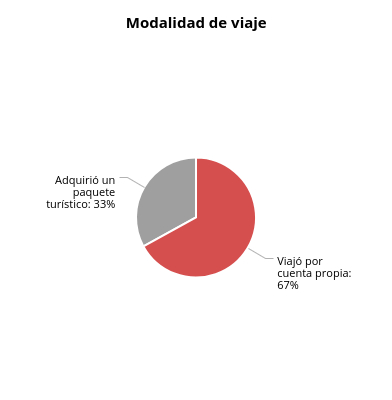
\includegraphics[scale=0.7]{Capitulo2/Figs/modalidad_viaje_extrajero.jpg}
    \caption{Porcentaje de modalidad de viaje de turista extranjero que visita Puno}
    \cite{2017PerfilExtranjerob}
    \label{fig:modalidad_viaje_extrajero}
\end{figure}

\begin{figure}[!ht]
    \centering
    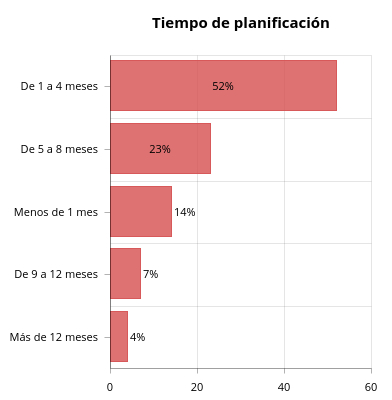
\includegraphics[scale=0.7]{Capitulo2/Figs/tiempo_planificacion_extranjero.jpg}
    \caption{Porcentaje de tiempo de planificación de viaje de turista extranjero que visita Puno}
    \cite{2017PerfilExtranjerob}
    \label{fig:tiempo_planificacion_extranjero}
\end{figure}

De acuerdo a otro reporte publicado también publicado por Promperú titulado “Perfil del Turista Nacional que visita Puno (2016)” se observa que en la organización de viajes el 99\% indica que viajó totalmente por cuenta propia (sin utilizar los servicios de una agencia de viaje / turismo) y un 1\% que compró un paquete turístico a una agencia de viajes / turismo en el lugar visitado. El 78\% no busca información, se pueden observar también que muchos de ellos no buscan ya que conocen el lugar (54\%) y algunos tienen referencia del lugar (25\%) mientras que un 22\% si busco información, entre los cuales podemos ver en la imagen 3, y la fuente de información podemos ver en la imagen 4.
\begin{figure}[!ht]
    \centering
    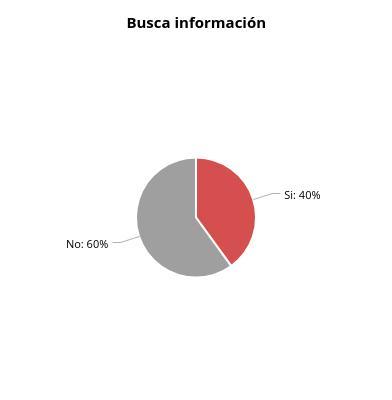
\includegraphics[scale=0.7]{Capitulo2/Figs/busca_informacion_nacional.jpg}
    \caption{Porcentaje que busca información de vacacionista nacional que visita Puno}
    \cite{2017PerfilNacional}
    \label{fig:busca_informacion_nacional}
\end{figure}

\begin{figure}[!ht]
    \centering
    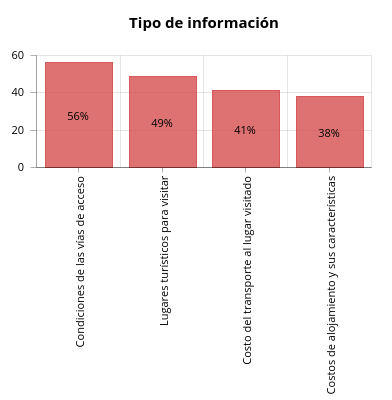
\includegraphics[scale=0.7]{Capitulo2/Figs/tipo_informacion_nacional.jpg}
    \caption{Porcentaje de tipo de información de vacionista nacional que visita Puno}
    \cite{2017PerfilNacional}
    \label{fig:tipo_infomacion_nacional}
\end{figure}

Como podemos ver en la imagen 3 la información que buscan los turistas nacionales son lugares turísticos a visitar en un 82\%, 70\% distancia y rutas de acceso, 66\% restaurantes donde acudir, 24\% costos de alojamiento y sus características, por lo tanto se ve que una solución como la que proponemos ayudará en la toma de decisiones en la planificación de itinerarios en la región Puno.

También al observar que los servicios de agencias de viajes ofrecen son transporte, alojamiento, alimentación, asistencia, etc. Y que los turistas prefieren opciones más personalizadas, en el trabajo que se realizará se considera que se hará un acercamiento a los servicios que brinda las agencias ya que como se puede observar en la imagen 3 las información que buscan lo turistas son relacionados, combinado con la personalización.

Trabajo en el futuro, que pueda cambiar en el momento el itinerario calculando nuevamente el itinerario, de esa manera se provee más flexibilidad.
\subsection{Social}
Esta investigación apoyará directamente al turista en la toma de decisiones en el diseño de un itinerario detallado para realizar de forma satisfactoria su viaje a la región de Puno, porque se consideran sus preferencias. Y los ciudadanos y los emprendedores de forma indirecta fortaleciendo la valoración cultural, la preservación del medio ambiente y el sentido de identidad nacional. 
\subsection{Económico}
Se considera también que ayudará a generar riquezas para el Perú en forma de impuestos. También se considera que minimizará el tiempo al turista al diseñar su viaje que al final se puede convertir en dinero.
\subsection{Ambiental}
Directamente se considera que ayudará en que se reduzcan el uso de papeles en la guías,etc., al usar la aplicación web. 
\subsection{Ciencia}
Se ha revisado que escasez de investigaciones en el Perú relacionados con el tema de planificación de viajes personalizados, en ALICIA, Repositorio Digital del CONCYTEC, en la cual será un aporte a la investigación en este tema. Así como también este trabajo al final al pedir información del turista recolecta información que servirá para un análisis.
Estudiar este tipo de problemas es una cuestión muy importe en computación y con muchas aplicaciones.\cite{Derivando2017QueYouTube}
\subsection{Legal}
Para generar políticas públicas a través del estado para que puedan ayudar a proteger los atractivos según la ley Nro. 29408 - Ley General de Turismo (2009).
\subsection{Ife}
El estudio por los algoritmos, la complejidad computacional que se puede ver que tiene varias aplicaciones y realizar una aplicación que se va a mejorar a través de la retroalimentación que se vaya investigando e implementando. 
\section{Presunción filosófica}
w
El avance de la tecnología, Dios